\documentclass[a4paper, 10pt]{report}

\usepackage[right=1in, left=1in, top=1in, bottom=1in]{geometry}
\linespread{1.5}
\usepackage{amsmath, amsthm, amssymb} %math's packages
\usepackage[utf8]{inputenc} %document encoding

\usepackage{amsmath, amsthm, amssymb}
\usepackage{enumerate}
\usepackage{verbatim}
%\usepackage{indentfirst}
\usepackage{graphicx}
\usepackage{algorithm}
\usepackage{algpseudocode}
\usepackage{listings}
\usepackage{color}
\usepackage{subcaption}
\usepackage{hyperref}
\usepackage{float}
\usepackage[T1]{fontenc}
\usepackage{makecell}
\usepackage{colortbl}
\usepackage{booktabs}
%\usepackage{babel}
\usepackage{array,multirow,graphicx}
\usepackage{tikz}
\usepackage[most]{tcolorbox} %using color boxes
\usepackage{pgfplots} %plots
\usepackage{standalone} %including other files without preambule
\usepackage{setspace}
\usepackage{tabu}

\usetikzlibrary{arrows.meta}
\hyphenation{distributions}
\usetikzlibrary{arrows, positioning, shapes.geometric}
\newtheoremstyle{break}% name
{}%         Space above, empty = `usual value'
{}%         Space below
{\itshape}% Body font
{}%         Indent amount (empty = no indent, \parindent = para indent)
{\bfseries}% Thm head font
{.}%        Punctuation after thm head
{\newline}% Space after thm head: \newline = linebreak
{}%         Thm head spec

\graphicspath{ {./Plots_transfer/} }
%\usepackage[svgnames]{xcolor}
%\usepackage[round]{natbib}


\newcommand{\cov}{\mathbb{C}\text{ov}}
\newcommand{\eig}{\text{EIG}}
\newcommand{\ape}{\text{APE}}
\newcommand{\kl}[2]{\text{KL}\left(\ #1\ ||\ #2\ \right)}
\newcommand{\entropy}[1]{H\left(\ #1\ \right)}
\newcommand{\expect}{\mathbb{E}}
\newcommand{\argmax}{\text{argmax}}
\newcommand{\simiid}{\overset{\text{\tiny iid}}{\sim}}
\newcommand{\qp}{q_p}
\newcommand{\qm}{q_m}
\newcommand{\ql}{q_\ell}
\newcommand{\R}{\mathbb{R}}
\newcommand{\prob}{\mathbb{P}}	
\newcommand{\tP}{\tilde{P}}	
\newcommand{\tPg}{\tilde{P}_{\gamma}}	
\newcommand{\tpi}{\tilde{\pi}}	
\newcommand{\tpig}{\tilde{\pi}_{\gamma}}
\newcommand{\tpigLi}{\tilde{P}_{\gamma,L,i}} 
\newcommand{\tpigLk}{\tilde{P}_{\gamma,L,k}} 
\newcommand{\tpigJi}{\tilde{P}_{\gamma,J,i}} 
\newcommand{\tpigJk}{\tilde{P}_{\gamma,J,k}} 
\newcommand{\RJi}{R_{\gamma,J,i}} 
\newcommand{\RJk}{R_{\gamma,J,k}}
\newcommand{\RLi}{R_{\gamma,L,i}} 
\newcommand{\RLk}{R_{\gamma,L,k}}
\newcommand{\Qgi}{Q_{\gamma,i}} 
\newcommand{\Qgk}{Q_{\gamma,k}}

\newcommand{\agi}{a_{\gamma,i}} 
\newcommand{\agk}{a_{\gamma,k}}  
\newcommand{\agj}{a_{\gamma,j}}  
\newcommand{\wgi}{w_{\gamma,i}} 
\newcommand{\wgk}{w_{\gamma,k}}
\newcommand{\wgj}{w_{\gamma,j}}
\newcommand{\giY}{\gamma \in \mathcal{Y}} 
\newcommand{\bb}[1]{\mathbb{#1}}
\theoremstyle{plain}
\newtheorem{thm}{Theorem}%[section]
\newtheorem{assu}[thm]{Assumption}
\newtheorem{prop}[thm]{Proposition}
\newtheorem{lemma}[thm]{Lemma}
\newtheorem{cor}[thm]{Corollary}
%
\theoremstyle{definition}
\newtheorem{ex}[thm]{Example}
\newtheorem{defi}[thm]{Definition}
\newtheorem{alg}{Algorithm}
%
\theoremstyle{remark}
\newtheorem{remark}[thm]{Remark}
\renewcommand{\baselinestretch}{1.5}

\begin{document}
	
	\documentclass[TRANSFER_THESIS.tex]{subfiles}
\begin{document}
\thispagestyle{empty}
\begin{titlepage}
\begin{center}
\hfill 
\includegraphics[width=2.0in]{figures/Dept_Stats_logo_vertical_CMYK.eps} \hfill . \\
\vspace{3cm}
\rule{150mm}{0.5mm} \\ [16pt]
\Huge Optimal experiment design
\rule{150mm}{0.5mm} \\ [4pt]
\vfill
\large \textsc{A thesis submitted in partial fulfillment of the requirements for \textit{transfer of status} from PRS to DPhil} \\
\vspace{1cm}
\large \textsc{November 2018} \\
\rule{\textwidth}{0.5mm} \\ [4pt]
{\fontsize{14}{14}\textsc{Adam Foster} \hfill \textsc{Department of Statistics}} \\ [8pt]
{\fontsize{14}{14} \textsc{University College \hfill University of Oxford}}
\rule{\textwidth}{0.5mm} \\ [4pt]
\end{center}
\vspace{2cm}
\end{titlepage}
\end{document}


	
	\tableofcontents
	
\newpage
	\chapter*{Acknowledgements}
	\addcontentsline{toc}{chapter}{Acknowledements}
	I have been fortunate, in the first year of my DPhil, to have worked with a number of brilliant people. First and foremost, I would like to acknowledge the support, advice and patience of my supervisor, Yee Whye Teh. Also within Oxford, both Benjamin Bloem-Reddy and Tom Rainforth have been incredibly generous with their time and expertise. Without them, I would have struggled to achieve much in my first year. I would also like to thank Emile Mathieu for his unwavering support and friendship. I am grateful to Noah Goodman for taking a gamble on an unknown DPhil student and supporting my application to Uber Technologies for an internship. Noah's enthusiasm and guidance made my internship a joy, and also set me on a new and exciting research path. I'd like to extend my thanks to Martin Jankowiak and Eli Bingham, as well as the whole pyro team, for their continued help and support.
	
	
	%The author would like to thank his supervisor, Professor , for his assistance and detailed feedback. 
	%\newpage
	
	\chapter*{Preface}
	\addcontentsline{toc}{chapter}{Preface}
	\label{chap:preface}
	This thesis aims to describe the current work I am undertaking in my DPhil and possible future directions that I may take on broadly related topics. Optimal experiment design only entered into my research in June 2018. The initial work in my DPhil related to a question posed to me by Yee Whye Teh, namely, `is probabilistic programming useful for Bayesian nonparametrics?'. Our NIPS workshop paper \cite{bnpppl} and our open source contributions to the language Turing were related to this question. Subsequently, I worked on a project with Benjamin Bloem-Reddy about Bayesian nonparametric models of networks which resulted in a UAI paper and oral presentation \cite{bntl}. During my internship at Uber and the past two months, I have worked on optimal experiment design. Chapter~\ref{chap:voed} will turn into a paper that we will submit to ICML 2019. We submitted a short version to the NIPS BDL workshop. Following ICML, I plan to continue research on optimal experiment design, as discussed in Chapter~\ref{chap:future}.
	
	\chapter{Introduction and literature review}
	\label{chap:intro}
	Much of machine learning is concerned with the analysis of given data. By contrast, the fields of optimal experiment design (OED) and active learning are concerned with the creation of new data by experimentation or query. In many contexts, careful design of the experiment leads to more efficient learning. The gain in efficiency can be dramatic -- rendering previously infeasible experimental programs feasible. (citation needed)

Idealised active learning can be represented as follows
\begin{center}
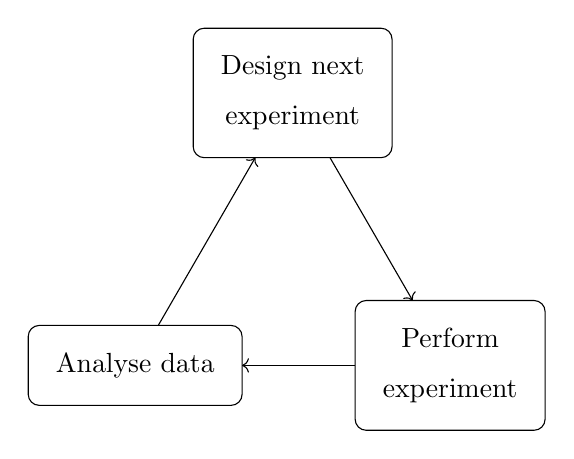
\begin{tikzpicture}
	[every node/.style={inner sep=10,outer sep=0,rounded corners}]
	\node (design) [draw, align=center] at (0, 0) {Design next \\ experiment};
	\node (perform) [draw, align=center] at (2, -3.46) {Perform \\ experiment};
	\node [draw] (analyse) at (-2, -3.46) {Analyse data};
	\draw [->] (design) -- (perform);
	\draw [->] (perform) -- (analyse);
	\draw [->] (analyse) -- (design);
\end{tikzpicture}
\end{center}
It is only within the context of a proposed data analysis that the optimality or suboptimality of an experiment design can be assessed.

\section{Foundations}
\subsection{Problem specification}
We assume the data analysis model for the experiment takes the form given by the graphical model
\begin{center}
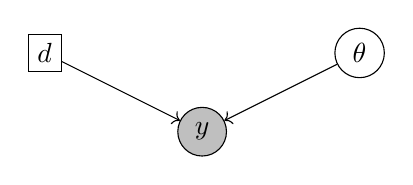
\begin{tikzpicture}
	\tikzstyle{every node}=[draw,shape=circle]
	\node[draw,fill=lightgray] (y) at (0, 0) {$y$};
	\node (t) at (2, 1) {$\theta$};
	\node[draw,shape=rectangle] (d) at (-2, 1) {$d$};
	\draw [->] (d) -- (y);
	\draw [->] (t) -- (y);
\end{tikzpicture}
\end{center}
in which $d$ represents the (non-random) design of the experiment, $\theta$ represents a latent variable and $y$ represents the observed outcome of the experiment. The joint density is
\begin{equation}
	p(y, \theta | d) = p(\theta)p(y|\theta,d)
\end{equation}
We can generalize to the sequential design setting by 
standard Bayesian updating, namely at experiment iteration $t$, we replace $p(\theta)$ with 
$p(\theta | d_{1:t-1}, y_{1:t-1})$, where $d_{1:t-1}$ and  $y_{1:t-1}$ are the designs and outcomes at previous steps of the experiment.
The likelihood $p(y_t | \theta, d_t)$ is assumed unchanged. That is, experimentation does not change the behaviour of the underlying system from time to time, conditional upon $\theta$.


\subsection{One-step design}
Suppose we assign a real-valued utility $U(y, \theta, d)$ to the event of observing $y$ under design $d$ when the true latent variable was $\theta$. We can average over $y$ to obtain
\begin{equation}
	U(\theta, d) = \int p(y | \theta, d)\ U(y, \theta, d)\ dy
\end{equation}
We can deal with $\theta$ in various ways
\begin{itemize}
	\item The Bayesian approach \cite{chaloner1995} places a prior $p(\theta)$ on $\theta$ and takes $U(d) = \int p(\theta)\ U(\theta, d)\ d\theta$
	\item The minimax approach \cite{fedorov1972} takes $U(d) = \inf_\theta U(\theta, d)$
	\item The local approach \cite{pronzato2010} begins with an estimate $\hat{\theta}$ and sets $U(d) = U(\hat{\theta}, d)$
\end{itemize}
The optimal design would then be
\begin{equation}
	d^* = \argmax_{d \in \mathcal{D}} \ U(d)
\end{equation}
where $\mathcal{D}$ is the space of admissible designs. Here, we primarily focus on the Bayesian approach. This is not an arbitrary decision, it can be motivated from decision theoretic considerations \cite{lindley1972}. See \cite{chaloner1995}, \cite{ryan2015} for further discussion of Bayesian experimental design.

Alternatively, we could take the (matrix-valued) `utility'
\begin{equation}
	U(y, \theta, d) = \left( \frac{\partial}{\partial \theta} \log p(y | \theta, d) \right)^2
\end{equation}
which leads to the the Fisher Information Matrix, used in many experiment design criteria \cite{pronzato2010}, defined as
\begin{equation}
	\mathcal{I}(\theta, d) = \int \left( \frac{\partial}{\partial \theta} \log p(y | \theta, d) \right)^2 p(y | \theta, d)\ dy
\end{equation}
We can obtain a scalar utility from $\mathcal{I}(\theta, d)$ by choosing from the `alphabetical' criteria \cite{box1982} which are defined as
\begin{itemize}
	\item D-optimality $U(d, \theta) = \text{det } \mathcal{I}(\theta, d)$
	\item A-optimality $U(d, \theta) = \text{tr } \mathcal{I}(\theta, d)$
	\item E-optimality $U(d, \theta) = \max_i \lambda_i$ where $\lambda_i$ are the eigenvalues of $\mathcal{I}(\theta, d)$
\end{itemize}

Work dating back to \cite{lindley1956} instead uses an information-theoretic utility\footnote{It can also be shown \cite{chaloner1995} that this utility leads to a (modified form) of D-optimality for linear models.}
\begin{equation}
	U(y, \theta, d) = \log \frac{p(\theta | y, d)}{p(\theta)} = \log \frac{p(y | \theta, d)}{p(y|d)}
\end{equation}
and Lindley established that this is the only form that satisfies certain intuitive properties of an informative experiment. For this reason, we will focus on this utility. See \cite{ryan2015} for a fuller discussion of utility functions used in experiment design.

With the information-theoretic utility and Bayesian averaging, we arrive at the following form for $U(d)$, called the \textbf{expected information gain (EIG)}
\begin{equation}
	U(d) = \eig(d) = \iint p(y, \theta | d) \log\frac{p(\theta | y, d)}{p(\theta)} \ dy\ d\theta
\end{equation}
The EIG can be interpreted in a number of ways
\begin{enumerate}
\item As the expectation of information gain. If we define
\begin{equation}
	\text{IG}(y, d) = \text{KL}(\ p(\theta | y, d)\ ||\ p(\theta)\ ) 
\end{equation}
then $\eig(d) = \expect_{y\sim p(y|d)}[\text{IG}(y, d)] $.
\item From APE. Define the \textbf{average posterior entropy} (APE) as 
\begin{align}
	\ape(d) &= \iint p(y, \theta | d) \log p(\theta | y, d) \ dy \ d\theta \\
	&= -\int p(y|d) \entropy{p(\theta | y, d)} dy
\end{align}
where $H$ is the differential entropy.
Then
\begin{equation}
	\eig(d) = \entropy{p(\theta)} - \ape(d)
\end{equation}
and the prior entropy is a constant w.r.t. $d$. Thus EIG maximisation corresponds to APE
minimisation.
\item Mutual information. Recall the mutual information is defined as
\begin{equation}
	\text{MI}(x, y) = \kl{p(x, y)}{p(x)p(y)}
\end{equation}
then we have
\begin{align}
	\text{MI}(y, \theta | d) &= \kl{p(y, \theta | d)}{p(y|d)p(\theta)} \\
	&= \iint p(y, \theta | d) \log \frac{p(y, \theta | d)}{p(\theta)p(y|d)} dy \, d\theta \\
	&= \eig(d)
\end{align}
\item Epistemic uncertainty.
The total entropy or uncertainty in response $y$ is
\begin{equation}
	\entropy{p(y|d)}
\end{equation}
the aleatoric uncertainty under parameter $\theta$ is
\begin{equation}
	\entropy{p(y|\theta, d)}
\end{equation}
Under prior $p(\theta)$, the expected aleatoric uncertainty is
\begin{equation}
	\expect_{\theta \sim p(\theta)}\left[ \entropy{p(y|\theta, d)} \right]
\end{equation}
The epistemic uncertainty, under $p(\theta)$, is
\begin{align}
	&\entropy{p(y|d)} - \expect_{\theta \sim p(\theta)}\left[ \entropy{p(y|\theta, d)} \right] \\
	=&-\int p(y|d)\log p(y|d)dy + \iint p(y, \theta | d)\log p(y|\theta, d) dy \, d\theta\\
	=& \eig(d)
\end{align}

\end{enumerate}
We shall see that the connection to mutual information in particular is handy for estimating EIG, because modern techniques for estimating MI have been developed in the recent past.


\subsection{Multi-step design}
Designing a sequence of multiple experiments, with a view to maximise expected utility can be viewed as a Partially Observable Markov Decision Process (POMDP), and falls within the scope of reinforcement learning \cite{pang2018}. The problem is also referred to as backward induction or stochastic dynamic programming. The formal reframing of OED as a POMDP is laid out below.

\subsubsection{Setup}
Suppose we have a determinic, finite time horizon $t=1, ..., T$. We specify as Partially Observable Markov Decision Process (POMDP) as follows.
\begin{itemize}
\item States $s_t = (\theta, h_t)$, where $h_t = d_{1:t}, y_{1:t}$ the history of designs $d$ and outcomes $y$ up to the current time. Here $y_t \sim p(y | \theta, d)$ is the outcome of performing the experiment using design $d_t$. The practical state $s'_t$ consists of the sufficient statistics for $\theta$ obtained from $h_t$. These can be used to compute the belief states $b_t$, encoding the full posterior for $\theta$ given that history $h_t$.
\item Actions $a_t = d_{t+1}$. Transitions correspond to running the experiment and producing the outcome $Y_{t+1}$.
\item Observations $o_t = h_t$. Thus the only unobserved part of the state $(\theta, h_t)$ is the latent $\theta$.
\item Rewards $r_t = r(t, \theta, h_t)$. We take $r$ to be a non-random function. Note that in many OED settings, we take $r_t = 0$ for $t<T$. Intuitively, this means we only care about our final understanding of or action upon the system, not the path taken to it. This is the choice made by \cite{gonzalez2016} among others.
\end{itemize}
Under this set-up, the \textit{optimal experiment design policy} is a $\pi$ from histories $h_t$ to actions $a_t$ which maximises the total reward
\begin{equation}
	R_T = \expect \left[ \sum_{t=1}^T \gamma^t r_t \mid \pi \right]
\end{equation}
where $\gamma \in [0,1]$ is the discount factor. In a finite horizon setting, we typically set this to 1. When there are only terminal rewards and $\gamma=1$, this reduces to
\begin{equation}
	\label{eq:terminalreward}
	R_T = \expect[r_T \mid \pi]
\end{equation}


\subsubsection{Connection to EIG}
\paragraph{Horizon 1}
Suppose $T=1$. Choose the following reward function
\begin{equation}
r(1, \theta, h) = \log \frac{p(\theta | y, d)}{p(\theta)} = \log \frac{p(y | \theta, d)}{p(y|d)}
\end{equation}
The $Q$-function of action $d_1$ is the expected reward
\begin{equation}
	Q(s_0, d_1) = E_{y \sim p(y|\theta, d)}[r(t, \theta, d_1, y)]
\end{equation}
Since we have no observation of $\theta$, the belief $Q$-function of the belief state $p(\theta)$ and action $d_1$ is
\begin{equation}
	Q(p(\theta), d_1) = E_{\theta \sim p(\theta)}\{E_{y \sim p(y|\theta, d)}[r(t, \theta, d_1, y)]\}
\end{equation}
which reduces to the familiar expression
\begin{equation}
	Q(p(\theta), d_1) = \iint p(y, \theta | d) \log \frac{p(\theta | y, d)}{p(\theta)} \, d\theta \, dy
\end{equation}

\paragraph{Horizon $T$}
This formalism provides a convenient way to avoid the greedy approach to sequential design that is compatible with the information-theoretic objective of \cite{lindley1956}.

Suppose the belief at time $t$ is $b_t(\theta)$. This can be computed from the sufficient stats $s'_t$. We take the reward to be $0$ at $t<T$ and
\begin{equation}
	r(T, \theta, h_T) = r(T, \theta, b_T(\theta)) = \log \frac{b_T(\theta) }{p(\theta)}
\end{equation}
we have updated $b$ according to Bayes Theorem so
\begin{equation}
	b_T(\theta) = p(\theta | y_{1:T}, d_{1:T})
\end{equation}
This reward structure represents the total information gained about $\theta$ from all experiments.

In fact, we can rewrite this reward to take non-zero values at earlier times, setting
\begin{equation}
	\label{eq:rlmutli}
	r(t, \theta, h_t) = r(t, \theta, b_t(\theta)) = \log\frac{b_t(\theta)}{b_{t-1}(\theta)}
\end{equation}
and this is equivalent to the previous formulation. To see this, consider the belief $Q$-function
\begin{align}
	Q(b_t(\theta), d_{t+1}) =& \int b_t(\theta)  \int p(y_{t+1} | \theta, d_{t+1}) \log\frac{b_{t+1}(\theta)}{b_t(\theta)} \\ &+ \int p(y_{t+2} | \theta, d_{t+1}, y_{t+1}) \log \frac{b_{t+2}(\theta)}{b_{t+1}(\theta)} + \hdots \, dy_{t+2} \, dy_{t+1} \, d\theta \\
	=& \int b_t(\theta) \int p(y_{t+1:t+2}|\theta, d_{t+1}) \log \frac{b_{t+2}(\theta)}{b_t(\theta)} + \hdots \, dy_{t+1:t+2} \, d\theta \\
	=& \hdots \\
	=& \int b_t(\theta) \int p(y_{t+1:T}|\theta,d_{t+1}) \log \frac{b_T(\theta)}{b_t(\theta)} \, dy_{t+1:T} \, d\theta
\end{align}
where $p(y_{t+1:T}|\theta, d_{t+1})$ assumes an optimal strategy after step $t+1$, under reward \eqref{eq:rlmutli}. We can now see by induction that the optimal strategy and $Q$-functions are the same for either choice of reward structure.

\subsubsection{The greedy approach}
In reinforcement learning, greediness refers to maximising the one-step-ahead reward, namely
\begin{equation}
	a_t = \argmax_{a_t \in \mathcal{A}} \left(\expect[r_{t+1} | a_t] \right)
\end{equation}
which, with the reward of \eqref{eq:rlmutli}, corresponds to one-step EIG maximisation at each step. We primarily focus on this form of multi-step optimisation because it removes all aspects of future planning beyond a single step from an already difficult problem.

\subsubsection{Non-greedy approaches}
Some have considered non-greedy strategies \cite{gonzalez2016} \cite{pang2018}. See \cite[sec 6.1]{ryan2015} for a summary of `backwards induction' approaches.


\subsubsection{Optional stopping}

We finally mention another possible complication. Rather than a fixed and finite time horizon $T$, we may we allowed to continue experimentation indefinitely, choosing when to stop. One natural choice to stopping criterion is to terminate when the posterior entropy reaches a threshold value.


\subsection{Theoretical considerations}
The proposed experimentation strategy in which we design future experiments on the basis of previous observations may, at first sight, cause some consternation to the theoretical statistician. The first question we seek to answer is `in what sense is the posterior obtained from multi-step OED the same as that obtained by a pre-ordained experimentation strategy?' The second line of questioning concerns the asymptotics of multi-step OED. `Is multi-step OED statistically consistent and does it provide a faster convergence rate than other methods?'

To the first question, the answer is simply that the posterior is the same as if the experimentation strategy had been pre-ordained. Indeed, let us regard the designs as random variables and consider a 2-step experiment with the following graphical model
\begin{center}
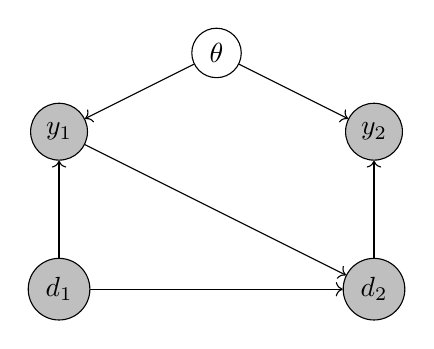
\begin{tikzpicture}
	\tikzstyle{every node}=[draw,shape=circle]
	\node (t) at (0, -1) {$\theta$};
	\node[draw,fill=lightgray] (y1) at (-2, -2) {$y_1$};
	\node[draw,fill=lightgray] (y2) at (2, -2) {$y_2$};
	\node[draw,fill=lightgray] (d1) at (-2, -4) {$d_1$};
	\node[draw,fill=lightgray] (d2) at (2, -4) {$d_2$};
	\draw [->] (d1) -- (y1);
	\draw [->] (t) -- (y1);
	\draw [->] (d2) -- (y2);
	\draw [->] (t) -- (y2);
	\draw [->] (d1) -- (d2);
	\draw [->] (y1) -- (d2);
\end{tikzpicture}
\end{center}
and the following conditional density for $\theta$
\begin{align}
	p(\theta | y_1, d_1, y_2, d_2) =& \frac{p(\theta, y_1, d_1, y_2, d_2)}{p(y_1, d_1, y_2, d_2)} \\
	=& \frac{p(\theta)p(d_1)p(y_1|\theta, d_1)p(d_2|y_1,d_1)p(y_2|\theta,d_2)}{\int p(\theta)p(d_1)p(y_1|\theta, d_1)p(d_2|y_1,d_1)p(y_2|\theta,d_2) d\theta} \\
	=& \frac{p(d_1)p(d_2|y_1,d_1)\ p(\theta)p(y_1|\theta, d_1)p(y_2|\theta,d_2)}{p(d_1)p(d_2|y_1,d_1)\ \int p(\theta)p(y_1|\theta, d_1)p(y_2|\theta,d_2) d\theta} \\
	=& \frac{p(\theta)p(y_1|\theta, d_1)p(y_2|\theta,d_2)}{\int p(\theta)p(y_1|\theta, d_1)p(y_2|\theta,d_2) d\theta}
\end{align}
showing that the dependence between $d_2$ and $d_1, y_1$ need not bother us. A related question from \cite{berry1985} was whether the map that takes the observed data to the posterior is a measurable function. This was addressed in \cite[pp. 18-20]{berry1985} in the restricted setting of the multi-armed bandit.

A powerful answer to the second question was given by \cite{paninski2005} and is a form of Bernstein--von Mises Theorem for EIG maximisation OED. Under relatively mild conditions, for any neighbourhood $\mathcal{U}$ of the true parameter value $\theta_0$ we have
\begin{equation}
	p(\mathcal{U} | y_{1:T}, d_{1:T}) \to 1 \text{ as } T \to \infty \text{ in probability}
\end{equation}
Under further conditions, we can show that the posteriors $p(\theta | y_{1:T}, d_{1:T})$ are asymptotically Normal with covariance matrix $\Sigma_\text{info}$. The same result holds for i.i.d. sampling of designs, giving rise to $\Sigma_\text{iid}$. We have that $\text{det}\ \Sigma_\text{info} \le \text{det}\ \Sigma_\text{iid}$. This led \cite{paninski2005} to say ``Thus, information maximization is in a rigorous sense asymptotically more efficient than the i.i.d. sampling strategy.'' Related results were obtained by \cite{pronzato2010} and \cite{hu1998}.

\section{Estimation of EIG}
The estimation of EIG, and quantities mathematically equivalent to it, has received attention from a diverse group of researchers.

\subsection{Challenges in EIG estimation}
Recall
\begin{align}
	\label{eig:post}
	\eig(d) =
	\iint  p(y, \theta | d) \log \frac{p(\theta | y, d)}{p(\theta)} \, dy\,  d\theta
	=\iint  p(y, \theta | d) \log \frac{p(y | \theta, d)}{p(y|d)} \, dy\,  d\theta.
\end{align}
The computation of this integral is challenging since neither $p(\theta|y,d)$ nor $p(y|d)$ nor the outer integral can, in general, be found in closed form.

A further complication arises when the likelihood $p(y|\theta,d)$ cannot be computed pointwise. For example, this is the case in the presence of nuisance variables, also known as random effects. 
These are additional latent variables, $\psi$, that we do not consider variables of interest and so we do not want to waste resources reducing our uncertainty for them. 
Such models arise frequently in scientific applications, for instance accounting for individual variation between participants in a survey. With random effects $\psi$ we have
\begin{equation}
	p(y|\theta, d) = \int p(y|\theta, \psi, d) p(\psi | \theta) d\psi
\end{equation}
which is typically intractable.

We survey existing approaches to EIG estimation.

\subsection{Nested Monte Carlo}
The estimator of \cite{vincent2017} and \cite{myung2013}, among others, is a nested Monte Carlo (NMC) estimator
\begin{equation}
	\eig(d) \approx \frac{1}{N}\sum_{n=1}^N \left[ \log p(y_n | \theta_n, d) - \log \left(\frac{1}{M} \sum_{m=1}^M p(y_n | \theta_m, d) \right) \right]
\end{equation}
where
\begin{align}
	y_n, \theta_n \simiid & \ p(y, \theta | d) \\
	\theta_m \simiid & \ p(\theta)
\end{align}
are all independent.

The drawbacks of such an estimator were noted in \cite{nmc}. Most notably, while simple Monte Carlo estimators converge with a mean squared error rate $\mathcal{O}(N^{-1})$ in the total number of samples, NMC estimators converge at a much slower $\mathcal{O}(N^{-2/3})$ rate and are biased, though consistent \cite{nmc}.

A saving grace of the MC approach is a speed-up due to \cite{vincent2017} in the case that $\mathcal{Y}$, the sample space of $y$, is finite. Then
\begin{equation}
	\eig(d) \approx \sum_y \left[ \frac{1}{N}\sum_{n=1}^N p(y | \theta_n, d) \log p(y | \theta_n, d) -  \left(\frac{1}{N} \sum_{n=1}^N p(y | \theta_n, d) \right) \log \left( \frac{1}{N} \sum_{n=1}^N p(y | \theta_n, d) \right) \right]
\end{equation}
where
\begin{equation}
	\theta_n \simiid \ p(\theta).
\end{equation}
Since this is a continuous function of vanilla Monte Carlo estimators, it converges at a rate $\mathcal{O}(N^{-1})$.

We finally mention that, whilst not present in the literature, NMC can be readily extended to the case of random effects
\begin{equation}
	\eig(d) \approx \frac{1}{N}\sum_{n=1}^N \left[ \log \left(\frac{1}{M'} \sum_{m'=1}^{M'} p(y_n | \theta_n, \psi_{nm'}, d) \right) - \log \left(\frac{1}{M} \sum_{m=1}^M p(y_n | \theta_m, \psi_m, d) \right) \right]
\end{equation}
where
\begin{align}
	y_n, \theta_n \simiid & \ p(y, \theta | d) \\
	\psi_{nm'} | \theta_n \sim & \ p(\psi | \theta_n) \\
	\theta_m, \psi_m \simiid & \ p(\theta, \psi)
\end{align}
and we note that we can replace $\psi_{nm'}$ with $\psi_m$ when $\theta$ and $\psi$ are independent under the prior $p(\theta, \psi)$. Again, when $\mathcal{Y}$ is finite a speed-up is possible, although we can no longer avoid nesting Monte Carlo estimators.

\subsection{Inference based approaches}
A number of authors \cite{long2013, ryan2015} use some form of Laplace approximation to $p(\theta|y,d)$ to estimate expected information gain. In \cite{ouyang2016}, probabilistic programming is used to completely solve the inference problem (in finite spaces) en route to estimating EIG.

\subsection{Mutual information estimation}
As mentioned previously, EIG estimation is mathematically equivalent to mutual information estimation, a topic that has received recent attention in part due to the connection with Generative Adversarial Networks (GANs) \cite{infogan} and disentanglement \cite{tianqichen}. In the following section, we drop $d$ from our graphical model, and consider a joint density $p(y, \theta) = p(\theta)p(y|\theta)$.

Since $p(\theta|y)$ is typically an intractable, we might use an approximation $q(\theta|y)$. An idea used by \cite{ba} and \cite{infogan} is to bound the mutual information in terms of an amortised posterior $q(\theta|y)$ as
\begin{align}
	\text{MI}(y, \theta) =& \int p(\theta) \int p(y|\theta) \log \frac{p(\theta | y)}{p(\theta)} \, dy \, d\theta \\
	\ge & \int p(\theta) \int p(y|\theta) \log \frac{q(\theta | y)}{p(\theta)} \, dy \, d\theta.
\end{align}
For a fuller derivation and discussion of this and related bounds, see Chapter~\ref{chap:voed} on variational optimal experiment design.

A more recent idea is to use the Donsker-Varadhan Representation of the KL divergence to estimate mutual information \cite{mine}. We have
\begin{equation}
	\label{eq:dv}
	\text{MI}(y, \theta) = \kl{p(y, \theta)}{p(y)p(\theta)} = \sup_T \left\{ \expect_{p(y,\theta)} [T(y, \theta)] - \log\left(\expect_{p(\theta)p(y)}[e^{T(y,\theta)}] \right)  \right\}
\end{equation}
where the supremum is taken over measurable $T$. Note that the optimising $T$ is given by
\begin{equation}
	T^*(y, \theta) = \log\frac{p(y,\theta)}{p(y)p(\theta)} + C \text{ where }C\text{ is any constant}
\end{equation}
The importance of \eqref{eq:dv} is that we no longer need access to any densities to estimate the mutual information.

Practical implementations arising from both these objective functions follow from choosing a suitable parametric family for $T$ (or, in the former case, for $q(\theta|y)$). One then optimises the bound w.r.t. the parameters of the family using finite sample approximations to the expectations. We note that such an idea is intimately connected with the GAN \cite{fgan}.

\section{Optimisation of EIG}
So far, little attention has been paid to the design $d$. We suppose now that $d \in \mathcal{D}$ and we seek
\begin{equation}
	d^* = \argmax_{d\in\mathcal{D}} \quad \eig(d)
\end{equation}
the optimal design. As outlined in the previous section, we can have only approximate estimates of $\eig(d)$. This puts us squarely in the domain of Bayesian optimisation \cite{shahriari2016}. When $\mathcal{D}$ is finite, we would term it a multi-armed bandit problem.

Bayesian optimisation in its simplest form requires
\begin{enumerate}
	\item A model of the unknown function
	\item An acquisition rule to decide which design(s) should be queried at the next iteration
\end{enumerate}
It is a fascinating fact that we are now back in the setting of OED. The variable of interest is the location of $d^*$, the maximiser of the unknown function. Other features of the function can be regarded as random effects. See \cite{pes} for further discussion on the connection between Bayesian optimisation and OED, in particular, the connection of EIG to Bayesian optimisation.

A popular approach to Bayesian optimisation is to choose a Gaussian process (GP) model of the unknown function, and an upper confidence bound (UCB) acquisition rule \cite{srinivas2009}.

One aspect that sets $\eig$ maximisation apart from conventional Bayesian optimisation is the ability for us to obtain more accurate estimates of the unknown function $\eig$ by varying the amount of computational resources assigned to estimation. This was explored by \cite{vincent2017} in a finite $\mathcal{D}$ setting. The number of NMC samples was increased for the most promising designs. \cite{mcleod2017} tackled a more general problem of variable cost objectives, taking a GP based approach.

\section{Applications}
TODO: Major revisions needed

\subsubsection{Machine learning and statistics}
There is long-standing interest in `classical' statistical models and their design \cite{youssefreview}. Consider a basic linear models with Gaussian noise. Optimal design here can be expressed in terms of the eigenspectrum of $XX^T$ (see \cite{chaloner1984}). For nonlinear models, see the section on Physics. What about GLMs? Likely can solve the problem analytically again. These are great baselines. People in the linear models case are often concerned with proving the equivalence of different kinds of optimality \cite{youssefreview}.

In machine learning, experiment design is closely related to two common techniques in, for example, image classification: data augmentation and active learning.

In data augmentation images are rotated, translated, etc to create more training data. We could theoretically optimise the augmentation but this seems wasteful since copying the labels to new images is very easy.

A much more interesting area is \textit{active learning}. In this context, there are a large number of unlabeled images. Labeling is expensive. We select which images to label either up front, or (more typical in active learning) in a sequential manner. The key difference here is that we have a finite pool of unlabeled instances. We may be more interested in reducing uncertainty in the labels of these unlabeled images than in our posterior entropy.

The connection between active learning and Bayesian optimal design was explored in \cite{golovin2010}. In this paper, they start from a place where the outcome of a test is deterministic (think of the 12 men on an island problem). In the noiseless setting, the sequential design can be encoded as a decision tree and the problem is called the Optimal Decision Tree problem. This problem is known to be NP-hard. The OED criterion is introduced later to account for noisy observations and the fact that true parameters need not be known exactly even after all tests have been run.

A particular active learning example can be found in \cite{nowak2009}. We have $\mathcal{H}$ a hypothesis space (read parameter space) and $\mathcal{X}$ a query space (read design space). The goal is to determine the true $h^* \in \mathcal{H}$. Each query outputs a label in $\{-1, 1\}$ corrupted with Bernoulli noise (independent between queries). The algorithm broadly works by targeting $x \in \mathcal{X}$ where the expected posterior label in near $0$ (random guess). The convergence rate of $\prob(\hat{h}_i \ne h^*) \to 0$ is studied (shown exponential). The importance of having access to unlabeled data is exploited by \cite{dasgupta2006}.

\subsubsection{Psychology}
For an overview of optimal experiment design in probabilistic programming, \cite{ouyang2016} from Noah's group is a good place to start. Experiment design is necessary to distinguish competing theories. We should select models with the highest \textit{expected information gain}, written formally as 
\begin{equation}
U(d) = \expect_{(Y, \Theta) \sim p(y, \theta | d)}\left\{\log \frac{p(\Theta | Y, d)}{p(\Theta)}\right\}
\end{equation}
This equation has been studied by mathematical statisticians since the 50's \cite{lindley1956}. We can naively evaluate $U(d)$ in a PPL via \textit{nested inference}.

A canonical experiment discussed in this paper is the 5-4 experiment for category learning \cite{medin1978}. The experiment aimed to distinguish two competing models of category learning: the \textit{exemplar model} (learn categories by comparing new items to all previous items) and the \textit{prototype model} (learn categories by remembering a prototypical example). There are two models, so $\Theta = \{m_1, m_2\}$. During the experiment, participants are presented with a sequence of objects. In the training phase, they are also told the correct label after guessing. In testing they have no feedback. The objects varied in four dimensions: colour, shape, size and count; we can consider the space of objects to be $\{0,1\}^4$. Each object has a label $A$ or $B$. The true labeling mechanism was limited by Medin and Schaffer to be linearly separable. There are 9 inputs in the final testing set and Medin and Schaffer restricted there to be 5 $A$s and 4 $B$s. The objects $0000$ and $1111$ have to be present. Under these restrictions there are 933 possible experiments up to permutation. So $\mathcal{D}$ is a finite set of size 933. $\mathcal{Y}$ is the `test' responses, ie. the subjects responses when they are not given feedback. Thus $\mathcal{Y} = \{A, B\}^9$. The kind of participant numbers seen were 10-30.

In \cite{vincent2017}, the canonical experiment is as follows. We want to model how humans discount future rewards relative to present ones (via utility indifference pricing framework). A single experiment takes the following form: `Would you prefer £$A_1$ at time $t_1$ or £$A_2$ at time $t_2$'? The parameter of interest is the discount factor. Formally, $\mathcal{D} = [0, \infty)^2$, $\mathcal{Y} = \{1, 2\}$ and $\Theta = [0, \infty)$. These three spaces fit together as follows. We first chose $\mathcal{D}$ the space of possible designs. We subsequently chose $\mathcal{Y}$ the space of possible outcomes. We posited a probabilistic model for $Y$ in terms of parameters $\theta$. Focus on non-nested estimation for finite $\mathcal{Y}$ and sequential design. Sequential design means different participants will be asked different questions based on their previous answers.

\subsubsection{Bioinformatics}

In \cite{vanlier2012}, the authors consider experiment design from the perspective that, with little data, many different parameter settings adequately describe the data. Canonical model. Biochemical network modeled as an ODE.
\begin{align*}
&\dot{x} = f(x, u, p) \\
&\dot{y} = g(x, q) + \xi \\
&x(0) = x_0
\end{align*}
$u$ is the input, $x, y$ are time varying (uncontrolled) with $x$ latent and $y$ observed, $p, q, x_0$ are parameters $\theta$ required to simulate the model and do not depend on $t$, $\xi$ represents measurement noise. We treat $\xi$ as iid Gaussian. The paradigm chosen here is expected variance reduction, as opposed to information gain. (Possibly wrong if people still do that.) The variance is in the posterior predictive density.

\subsubsection{Physics}
In \cite{berg2003}, we begin by discussing `classical' experiment design procedures which assume linear dependence between model and outcome $y = G_{m_0}d$. One can solve this linear equation by least squares, $\hat{d} = G^T(GG^T)^{-1}y$. Define $L = G^T(GG^T)^{-1}$, possibly adding regularization as necessary. Basically, you want to maximize the max eigenvalue of $G$, which is essentially a gradient. The larger gradient, the more informative the experiment. In a linear setting, the gradient does not depend on the true parameter value.

Now consider linear noise but a nonlinear function between parameters and outcomes. For example, the authors took
\begin{equation}
R_p = \left(\frac{1}{2}[1 + \tan^{-1} i] - 4c^2 \sin^2 i\right) \frac{\Delta \alpha}{\alpha}
\end{equation}
where $\alpha = (\alpha 1 + \alpha2)/2$, $\Delta \alpha = (\alpha 2 - \alpha 1)$. The parameter we want to optimize is $\alpha2$.

This is a relatively simple and comprehensible case.
	
	\chapter{Estimating EIG}
	\label{chap:voed}
	\textbf{Note}: This chapter is broadly based on a paper recently submitted to the NIPS BDL workshop; we intend to submit a longer version to ICML 2019.
\bigskip

As outlined in Sections~\ref{sec:esteig} and~\ref{sec:opteig}, the main technical barriers to OED using EIG maximisation are the estimation and optimisation of EIG.

The core contribution of this chapter is to introduce efficient variational methods for EIG estimation that are applicable to a wide variety of models.
The first method, which is related to amortised variational inference \cite{dayan1995helmholtz,kingma2014auto,paige2016inference,rezende2014stochastic,stuhlmuller2013learning}, employs an approximate posterior distribution, parameterised by the design and the experimental outcome. In a similar manner the second method employs a variational distribution for the marginal density over experimental outcomes for a given design. 
%{\bf [Eli:  define amortised - is there a classical OED or BDT-flavored reference that would serve as a nice foil against which to explain the value of amortisation?]}
Both methods can benefit from recent advances in defining flexible families of amortised variational distributions 
using neural networks (e.g.~normalising flows \cite{rezende2015variational,tabak2013family}). For this reason we developed our system in Pyro \cite{pyro}, a deep probabilistic programming language that provides first class support for neural networks and variational methods.  

The Nested Monte Carlo (NMC) approach (see Section~\ref{sec:nmc}) is inefficient because it constructs an independent estimate of $p(\theta | y, d)$ or $p(y|d)$ for each outcome $y$.
Our key insight is that by taking a variational approach, we can instead learn an \emph{amortized} approximation
for either $p(\theta|y,d)$ or $p(y|d)$, and then use this approximation to efficiently estimate the EIG.  In
essence, the estimate of $p(y_1|d)$ provides information about $p(y_2|d)$ for similar $y_1$ and $y_2$ (presuming
the density is smooth) and so it is more efficient to learn the functional form for $p(y|d)$ (or $p(\theta|y,d)$),
than to treat separate values of $y$ as distinct inference problems.

\subsection{Bounding EIG}
We construct a variational bound, $\mathcal{L}_p(d)$, using the amortized posterior $\qp(\theta | y,d)$:
\begin{align}
	\eig(d) =& \iint  p(y, \theta | d) \log \frac{p(\theta | y, d)q_{{p}}(\theta | y,d)}{\qp(\theta | y,d)} \, dy \, d\theta + \entropy{p(\theta)}  \\
	=& \iint p(y, \theta | d) \log \qp(\theta | y, d)  \, dy\, d\theta+\entropy{p(\theta)} + \mathbb{E}_{p(y|d)} \left[\text{KL}\left(p(\theta | y,d)||\qp(\theta | y, d)\right)\right]\\
	\label{eq:postbound}
	\ge& \iint p(y, \theta | d) \log \qp(\theta | y, d) \, dy\, d\theta+\entropy{p(\theta)} \triangleq \mathcal{L}_p(d).
\end{align}
%%%
In analogy with variational inference, this bound is tight when $\qp(\theta | y, d) = p(\theta | y, d)$.
%
Alternatively, we can instead introduce a marginal density $\qm(y|d)$, which results in an upper bound $\mathcal{U}_m(d)$:
%%%
\begin{align}
	\eig(d)&= \iint p(y, \theta | d) \log p(y | \theta, d) \, dy\, d\theta-\int p(y|d) \log \frac{p(y|d)\qm(y|d)}{\qm(y|d)} dy
	\\
	=& \iint p(y, \theta | d) \log p(y | \theta, d) \, dy\, d\theta-\int p(y|d) \log \qm(y|d) \, dy
	-\text{KL}\left(p(y|d)||\qm(y|d)\right)\\
	\label{eq:margbound}
	\le& \iint p(y, \theta | d) \log p(y | \theta, d) \, dy\, d\theta-\int p(y|d) \log \qm(y|d) \, dy
	\triangleq \mathcal{U}_m(d),
\end{align}
%%%
where the bound becomes tight for $\qm(y|d)=p(y|d)$.

\subsection{Estimation}
Just as in variational inference, the bounds in the previous section can be maximised with stochastic gradient methods \cite{robbins1951stochastic}. Concretely, suppose $\mathcal{Q}$ is a family of amortised variational approximations $\qp(\theta | y, d; \phi)$  indexed by $\phi$. We can estimate EIG by maximizing the lower bound $\mathcal{L}_p(d;\phi)$:
%%%
\begin{equation}
	\label{eq:maxpost}
	\text{EIG}(d) \approx \max_\phi \mathcal{L}_p(d;\phi) =
	\max_\phi \left\{ \int p(y, \theta | d) \log \qp (\theta | y, d; \phi)\, dy\, d\theta  \right\} + \entropy{p(\theta)}
\end{equation}
%%%
To do so only requires  that we can generate samples from the model,
$y_i, \theta_i \sim p(y, \theta | d)$; 
in a probabilistic programming context this corresponds to running the model forwards with no conditioning.
We can then construct the required Monte Carlo estimates for the gradient as
\begin{equation}
\nabla_{\phi} \mathcal{L}_p(d;\phi) \approx \nabla_\phi \left\{\frac{1}{N}\sum_{i=1}^N \log \qp(\theta_i|y_i, d; \phi)\right\} \quad \text{where} \quad y_i, \theta_i \overset{\tiny{\text{i.i.d.}}}{\sim} p(y, \theta | d),
\end{equation}
%\begin{equation}
%\nabla_{\phi} \mathcal{L}_p(d;\phi) \approx \nabla_\phi \left\{\frac{1}{N}\sum_{i=1}^N \log \qp(\theta_i|y_i, d; \phi) - \frac{1}{N} \sum_{i=1}^N \log p(\theta_i)\right\} \quad \text{where} \quad y_i, \theta_i \overset{\tiny{\text{i.i.d.}}}{\sim} p(y, \theta | d),
%\end{equation}
noting that no re-parameterization is required as $p(y,\theta|d)$ is independent of $\phi$.
An analogous scheme can be constructed for the upper bound $\mathcal{U}_m(d;\phi)$, expect that we now
perform a minimization.


\subsection{Accounting for random effects}
Note that the lower bound $\mathcal{L}_p(d)$ can be computed whether or not the model contains random effects (see Section~\ref{sec:challenges} for a discussion of random effects). On the other hand, the definition of $\mathcal{U}_m(d)$ involves $p(y|\theta,d)$ which is typically intractable in the case of random effects.

Fortunately, we can still make progress. Starting from
\begin{equation}
\label{eq:EIGp-app}
	\eig(d) = \iint  p(y, \theta | d) \log p(y|\theta, d) dy\,d\theta - \int p(y | d) \log p(y | d) dy
\end{equation}
and we can bound each term separately in terms of two approximate densities: $\qm(y|d)$ for the marginal and $\ql(y|\theta,d)$ for the likelihood. Specifically,
we have from Gibbs' inequality
\begin{align}
	-\int p(y | d) \log p(y | d) dy &\le -\int  p(y|d)\log \qm(y|d) dy \\
	\iint p(y, \theta |d) \log p(y|\theta,d) dy\,d\theta & \ge \iint p(y, \theta, | d) \log \ql(y|\theta, d) dy\,d\theta \,.
\end{align}
%%%
Here we can no longer derive a direct bound on the EIG, but we can still
use these inequalities to train to amortized densities, which will yield the
true EIG if they match the true densities.
Namely, suppose $\mathcal{Q}_1$ is a family of variational distributions  $\qm(y|d; \phi_1)$ indexed by $\phi_1$ 
and $\mathcal{Q}_2$ is a family of variational distributions $\ql(y|\theta,d; \phi_2)$ indexed by $\phi_2$. Then a suitable objective for learning $\phi_1, \phi_2$ is
\begin{align}
\mathcal{D}_{\phi_1, \phi_2}(d) &\triangleq
- \iint  p(y, \theta, | d) \log \ql(y|\theta, d; \phi_2)dy\,d\theta 
-\int p(y | d) \log \qm(y | d; \phi_1)dy  \\
\{\phi_1^*, \phi_2^*\}	&= \text{argmin}_{\phi_1, \phi_2} \mathcal{D}_{\phi_1, \phi_2}(d)
	\end{align}
where the optimization can be performed using stochastic gradient methods, as in the main paper. Once these approximations have been learned, we can plug
them back into~\eqref{eq:EIGp-app} to give
\begin{equation}
	 \eig(d) \approx  \iint  p(y, \theta, | d)\log \ql(y|\theta, d; \phi_2^*) dy\,d\theta 
	 -\int p(y | d) \log \qm(y | d; \phi_1^*) dy
\end{equation}
which can then itself be approximated by conventional Monte Carlo
sampling.

\subsection{Experiments}
\label{sec:experiments}

We validate our EIG estimators on a selection of generalized linear models. These serve as useful benchmarks, since they are workhorse models in many different scientific disciplines. Our results are summarized in Table~\ref{tab:abserrors} and Fig.~\ref{fig:lm}-\ref{fig:nig}. In all four cases, both estimators
(i.e.~the posterior method based on $\qp$ and the marginal method\footnote{correcting for random effects as necessary} based on $\qm$) 
gave significantly lower variance than the NMC baseline, and in all but one case a
significantly lower bias as well. We note that NMC especially struggles with random effects (LinReg + RE). More worryingly still, the bias of the NMC estimator can exhibit strong systematic variation as a function of the design, see Fig.~\ref{fig:lm}-\ref{fig:nig}. This is problematic because it can lead to the choice of a significantly suboptimal design. It is also worth emphasizing the utility of having multiple variational methods at our disposal: while the marginal method yields poor EIG estimates for the model with a large output dimension, the posterior method delivers high quality estimates. 
%On the other hand, the fact that the marginal method is an upper, rather than a lower, bound can be advantageous form an optimization perspective
%when making sequential decisions, as it is a naturally conservative choice.
% Finally, it is worth noting that our estimators can still yield good EIG estimates when the variational distribution is imperfectly specified (N$\Gamma^{-1}$Reg).
Finally, we consider an example (N$\Gamma^{-1}$Reg) that is not purely Gaussian. Here our method still performs well, despite the variational families not containing the true posterior or marginal.

%For a number of different EIG estimation tasks we compare: i) nested Monte Carlo (NMC), ii) our posterior method based on $\qp$, iii) our marginal method\footnote{with the correct correction for random effects when present, as detailed in Appendix~\ref{sec:margre}} based on $\qm$.
%
%Our first experiments was a linear regression model (LinReg) which has analytic EIG (enabling comparison of estimator accuracy). See Table~\ref{tab:abserrors} for the bias and variance of the estimators. Our methods strongly outperformed NMC, and also have the correct bias (negative bias for posterior, positive bias for marginal). Including random effects (LinReg + RE) didn't change this picture. Increasing $n$, the dimension of $y$, (LinReg large $n$) led to poorer performance in the marginal method -- likely because of the large number of parameters necessary to model $y|d$. To examine the effect of misspecified variational families, we changed the linear model to a Normal inverse Gamma (N$\Gamma^{-1}$Reg). As seen in Table~\ref{tab:abserrors}, the upper and lower bounds separate, but remain closer to the true answer than NMC.  Full details of the models and experiment set-up can be found in Appendix~\ref{sec:exp}.

\begin{table}[h!]
\begin{center}
    \begin{tabu}{|c|[1pt]c|c|c|c|c|c|c|c|}    \hline
  & \multicolumn{2}{c|}{\small LinReg} & \multicolumn{2}{c|}{\small LinReg + RE}  & \multicolumn{2}{c|}{\small LinReg large ${\rm dim}(y)$}  & \multicolumn{2}{c|}{\small N$\Gamma^{-1}$Reg}  \\  
  \hline
  & \small bias & \small var  & \small bias & \small var  & \small bias & \small var  & \small bias & \small var  \\
  \tabucline[1pt]{-}
   \small NMC & \small 1.37 & \small 1.93 & \small 5.33 & \small 3.84 & \small 3.13 & \small 2.97  & \small 3.39 & \small 3.20   \\ \hline
    \small Posterior & \small -0.23 & \small 0.25   & \small -0.55 & \small 0.41   & \small -0.29 & \small 0.31 & \small -0.50 & \small 0.51      \\ \hline
   \small Marginal & \small 0.34   &\small 0.15  & \small 0.36  &\small 0.20 &\small 4.57 & \small 0.29 & \small 1.59 & \small 0.64    \\ \hline
    \end{tabu}
\end{center}
     \caption{Bias and variance of EIG estimation averaged over 10 runs and 11 designs. Each method was run for 10 seconds. For more details on the models and experimental setup see Appendix~\ref{sec:expdeets}.  Note that the directions of the bias for the
     posterior and marginal match the fact that they are lower and upper bounds, as would be expected.
 \vspace{-10pt}}
     \label{tab:abserrors}
\end{table}

\begin{figure}[h]
	\begin{center}
		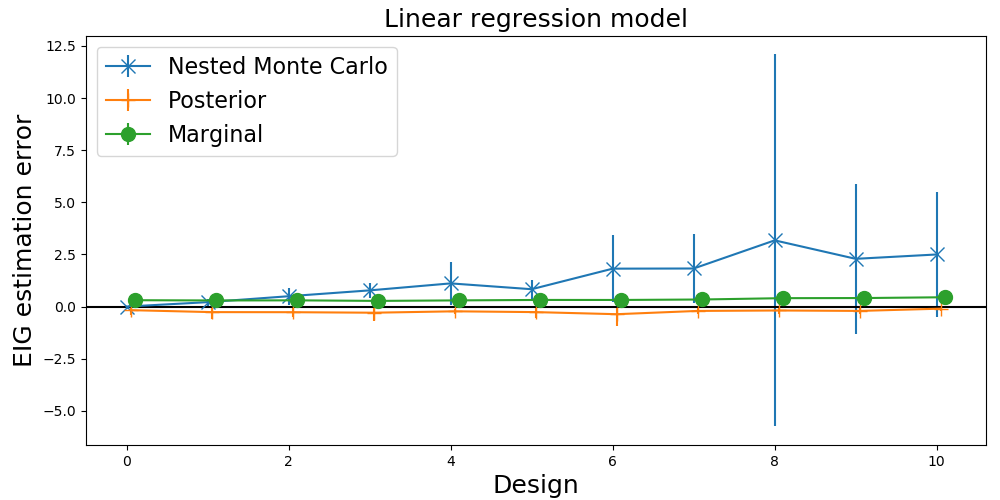
\includegraphics[scale=.5]{figures/lm.png}
	\end{center}
	\caption{LinReg: EIG estimates for a linear regression model over 11 designs. We plot the mean and twice the standard deviation from 10 runs. Computational time was set to 10 seconds for comparison.}
	\label{fig:lm}
\end{figure}

\begin{figure}[h]
	\begin{center}
		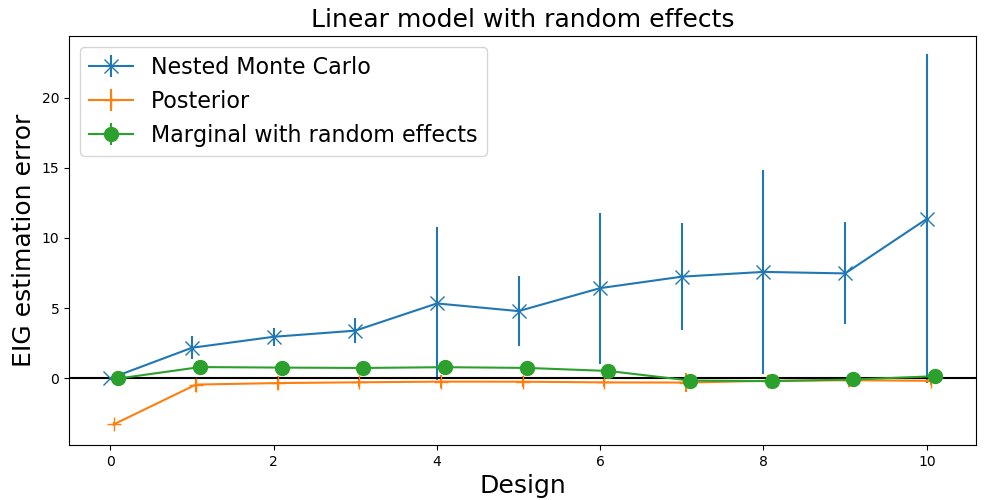
\includegraphics[scale=.5]{figures/lm_re.png}
	\end{center}
	\caption{LinReg + RE: EIG estimates for a linear regression model with random effects. Settings as in Figure~\ref{fig:lm}.}
	\label{fig:lm_re}
\end{figure}

\begin{figure}[h]\centering
	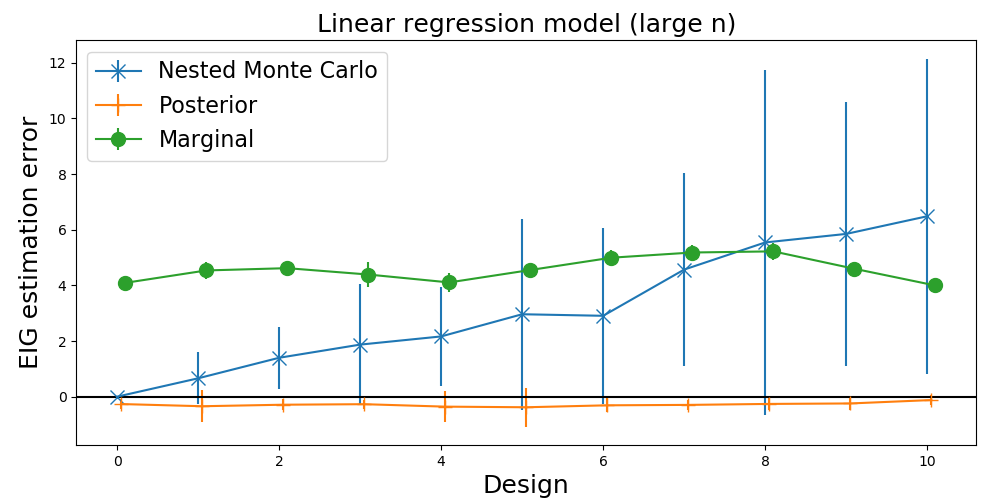
\includegraphics[scale=.5]{figures/lm_large_n.png}
	\caption{LinReg large ${\rm dim}(y)$: with settings as in Figure~\ref{fig:lm}.}
	\label{fig:largen}
\end{figure}

\begin{figure}[h]
	\begin{center}
		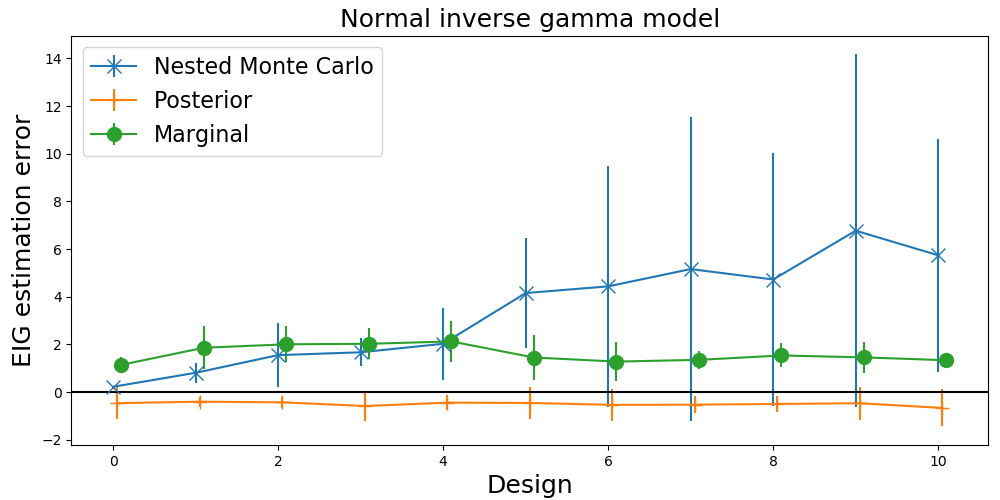
\includegraphics[scale=.5]{figures/nig.png}
	\end{center}
	\caption{N$\Gamma^{-1}$Reg: EIG estimates for a Normal inverse-Gamma model. Settings as in Figure~\ref{fig:lm}.}
	\label{fig:nig}
\end{figure}
	
	\chapter{Future directions}
	\label{chap:future}
	In this section, we outline ideas for future research in OED. Some ideas are clear next steps proceeding from the greedy EIG maximisation paradigm that has been adopted so far. The ultimate goal of this project would be a probabilistic programming framework that can efficiently design (near) optimal experiments for a wide variety of models and design spaces. There are also theoretical questions about this paradigm that ought to be addressed.

It is also possible to address shortcomings in the current framework. Non-greedy strategies, and experiment design with costs both connect with the POMDP formulation of the problem. The open question is how far we can maintain good performance whilst beginning to tackle these issues.

Moving beyond EIG entirely forces us to confront more fundamental questions of what practitioners need from experiment design. One aspect that is clearly important is the connection with causal inference -- indeed some scientists view avoiding false causal inferences as \textit{the} problem of experiment design, optimal or otherwise. Another issue of importance is model misspecification. EIG in some sense assumes that the model is exactly true. Would optimal design look the same if we admitted a probability that the model was incorrect? Suppose instead, we sought to design experiments that actively exposed flaws in the model.

With such a diversity of interesting questions in this area, the difficulty is prioritisation. So far, we have sought to strike the balance between building things that work efficiently on some problems, and maintaining generality and provable correctness. Potential applications, interest and advice will guide future priorities.


\section{Greedy EIG maximisation}
\subsection{Expanding the scope of variational OED}
Variational optimal experiment design as outlined in Chapter~\ref{chap:voed}, whilst a generally applicable idea, is currently limited in practice to (a subset of) GLMMs. The guides are highly structured and exploit knowledge of the models. If we are interested in OED for sequential human-in-the-loop experiments, there is a definite upper limit on acceptable computation time. This would encourage us to delve forwards with simpler models. The objective would be to drive computation down as far as possible.

On the other hand, our literature review highlighted the interest in a number of other more complex models. When experiments are very expensive or timely, there is scope to allow a much longer OED computation time. Among `complex' models, nonlinear regression models are foremost. We can broadly divide these into parametric models (e.g. the differential equation model of \cite{vanlier2012}) and Bayesian nonparametric models where the Gaussian process is the leading example. We should also distinguish between the Bayesian optimisation case --  in which the only quantity we are interested in is the location of the optimum -- and cases where we genuinely want to maximise information about the entire function. These two classes of nonlinear regression models suggest different variational approaches. For highly nonlinear parametric models, it is likely that we dispense with assuming any knowledge of the nonlinearities and fall back on flexible approximators like deep neural networks. Gaussian processes, on the other hand, have mathematical structure that can be exploited (e.g. \cite{pes}). Benchmarks, particularly for Bayesian optimisation, are likely to be harder to beat for the GP. The interest in such OED problems, though, is correspondingly high.

We could instead ask: in which cases does OED deliver the greatest benefit? That is, under which conditions would an experimental program without OED, or with inaccurate OED, be inefficient? A partial answer to this question can be given by the interpretation of EIG as epistemic uncertainty in the response (see Section~\ref{sec:onestep} for derivation)
\begin{equation}
	\eig(d) = \entropy{p(y|d)} - \expect_{p(\theta)}[\entropy{p(y|\theta,d)}].
\end{equation}
Thus $\eig(d)$ will be low whenever $p(y|d)$ is certain. This is intuitive -- if our current model already accurately predicts $y$ at query $d$, little we be gained from confirming that outcome. However, high uncertainty in $y|d$ is not enough. We also need the expected aleatoric uncertainty to be low. Put another way, if knowing the exact values of $\theta$ still fails to resolve the uncertainty in the outcome then querying at $d$ will not tell us much about $\theta$. We can manufacture interesting OED problems using these two insights. First, data censoring means that $\entropy{p(y|d)}$ will be low unless we avoid the censored region. Secondly, allowing the strength of random effects to be higher for some $d$ than others means $\entropy{p(y|\theta,d)}$ will be high unless we avoid the noisy region.

One possible problem to explore is modelling distances, for instance using multi-dimensional scaling \cite{torgerson1952multidimensional}. The design would be a pair $d = (x_1, x_2)$ of object to compare. This could become a very interesting problem if i) the response was censored for very dissimilar objects, ii) responses on previous objects allow us to accurately predict the outcome on some others. Both of these ideas could reduce $\entropy{p(y|d)}$ for certain designs. One specific application is in psychology when studying the similarity between concepts \cite{shepard1962analysis}.

\subsection{Importance weighting correction to variational OED}
The variational methods of Section~\ref{sec:voed} are biased and, if $\mathcal{Q}$ is chosen poorly, do not converge to the true EIG. NMC, though sometimes very slow, is a consistent procedure. We explore the connection between the two here. We have
\begin{equation}
	\eig(d) = \iint p(y, \theta | d) \log p(y|\theta, d) \, dy \, d\theta - \int p(y|d) \log \left( \int p(y|\theta,d) p(\theta) \, d\theta \right) \, dy
\end{equation}
and conventional NMC proceeds by estimating the integral $\int p(y|\theta,d) p(\theta) \, d\theta$ using fresh samples from $p(\theta)$. We could instead use $\qp(\theta|y,d)$ as a proposal
\begin{equation}
	\int p(y|\theta,d) p(\theta) \, d\theta = \int p(y|\theta,d) \frac{p(\theta)}{\qp(\theta|y,d)} \qp(\theta|y,d) \, d\theta.
\end{equation}
Using one Monte Carlo sample for this integral reduces to the estimators used in Section~\ref{sec:voed}. If we instead used $M$ samples, we would have a new NMC estimator
\begin{equation}
	\eig(d) \approx \frac{1}{N}\sum_{n=1}^N \left[ \log p(y_n | \theta_n, d) - \log \left(\frac{1}{M} \sum_{m=1}^M p(y_n | \theta_{nm}, d)\frac{p(\theta_{nm})}{\qp(\theta_{nm}|y_n,d)} \right) \right]
\end{equation}
where
\begin{align}
	y_n, \theta_n \simiid & \ p(y, \theta | d) \\
	\theta_{nm}|y_n \simiid & \ \qp(\theta|y_n,d).
\end{align}
and we would have a consistent estimator that likely converges much faster than conventional NMC. Note the connection with the IWAE \cite{iwae}, an importance weighting correction to the VAE ELBO.

It would also be interesting to see if we can find a correction that uses $\qm$, our approximation to the marginal, rather than $\qp$.


\subsection{Estimating the gradient of EIG}
Thus far, we have primarily focused on point estimation of $\eig(d)$. Many optimisation procedures (over $d$) rely instead on estimates of $\nabla_d\,\eig(d)$. We first note that, as $\eig$ is an expectation over $p(y,\theta|d)$, the reparametrization trick and its extensions \cite{tucker2017rebar, rezende2014stochastic} would be attractive here.

Suppose that we use our variational OED estimates in place of true EIG evaluations. Then the global optimisation problem tackled is
\begin{equation}
	\max_d \max_\phi \left\{ \iint p(y, \theta | d) \log \qp (\theta | y, d; \phi)\, dy\, d\theta  \right\} + \entropy{p(\theta)}.
\end{equation}
Rather than a lengthy process of optimising $\phi$ at each step, we could iterate between gradient steps in $\phi$ and $d$ space (or compute a combined gradient step) to reach the global optimum, as is done with the Generative Adversarial Network (GAN) \cite{goodfellow2014generative}. If successful, this approach could make finding local optima of $\eig$ computationally similar in difficulty to evaluating $\eig$ at a single point.
Alternatively, using gradient information within Gaussian process driven Bayesian optimisation \cite{osborne2009gaussian} is possible, and may be preferable in OED where a global optimum is desired.

\subsection{A sequential design framework in a probabilistic language}
Implementation in Pyro has so far focused on EIG estimation procedures. Building a general purpose toolkit for sequential OED remains a project of both software development and research. In such development, we would like to maintain the ability to change the EIG estimation and optimisation procedures relatively easily, including combining them as in the previous section. Part of the process that has not received a great deal of attention thus far is the sequential aspect of the problem. Having designed and performed an experiment, we need to compute the posterior on $\theta$, and then proceed using this as a new prior. When using posterior variational OED, that based on $\qp$, we will already have an approximation to the posterior. If sampling techniques (e.g. MCMC) are used to sample the posterior, we will no longer assume access to the density $p(\theta)$. Fortunately, this does not affect our current estimators: in one, the density is never used and in the other $\entropy{p(\theta)}$ is a constant in an optimisation problem that we can safely ignore. An approach using Population Monte Carlo (PMC) was outlined in \cite{vincent2017}.


\subsection{Optional stopping}
We conclude by outlining more theoretical directions we might wish to take. As was mentioned very briefly in Section~\ref{sec:optstop}, optional stopping might form part of sequential OED. Statistical analysis of optional stopping has a long history~\cite{chernoff1972sequential}. Which optional stopping rules are we allowed to use in EIG driven sequential experimentation with Bayesian data analysis? Bayesian analysis is concerned not only with testing hypotheses but also with establishing uncertainty. Which conclusions are we able to draw from our posterior when that posterior was created from optional stopping?


\subsection{EIG and power}
Frequentist statisticians typically design experiments using a notion of statistical power (that is tied to a specific hypothesis). What is the connection between EIG and power?

Our interest in information arises from a belief that optimising overall information will allow us to tackle many downstream tasks. We would like to make a statement like the following: `EIG optimisation is optimal when an unknown problem is to be solved using the final posterior'. Such a problem could be a hypothesis test. The connection with decision theory should also be explored.


\section{Beyond greedy EIG maximisation}
\subsection{Cost and non-greedy optimisation}
Frequently, experimentation is not free and the cost varies with the design. This is particularly the case when the magnitude of the experiment is a design parameter. With the inclusion of costs, we might wish to optimise
\begin{equation}
	U(d) = \eig(d) - \lambda C(d)
\end{equation}
where $C(d)$ is the cost of the design and $\lambda$ is a constant that determines the trade-off between information and cost.

When designing a single experiment, the inclusion of cost seems relatively simple. In the multi-step case, the inclusion of cost may be more important. For example, in a sequential design problem with costs and a finite horizon $T$, it would make sense to perform cheaper experiments at early times. Once some aspects of the system are understood, we can proceed to more expensive experiments with less risk of performing the wrong experiment. In the case of a fixed budget, we would be happy to use up our entire budget at time $T$, but would be much more cautious at time $1$.

Proceeding to the question of non-greedy optimisation more generally, it has been noted that we can view the problem as a POMDP and so generic methods like Partially Observable Monte Carlo Planning \cite{pomcp} are applicable. Suppose we wish to maximise total information gain, possibly including costs. Are there features of the problem that allow us to do significantly better than using generic POMDP solvers?

\subsection{Causal inference}
It is common in science that experiments are performed to learn causal structure or to estimate expectations defined using \textit{do}-calculus \cite{pearl2009causal} such as $\expect[Y | do(X=x)]$. Many flaws in scientific experiment design are the result, not of gaining too little information, but of making inappropriate causal assumptions or incorrectly estimating these sorts of expectations.

How does experiment design for causal inference intersect with experiment design for information? It is possible that causal statistics simply defines a subset $\mathcal{D}' \subseteq \mathcal{D}$ of designs that are valid from a causal inference perspective. We could then seek $\max_{d\in\mathcal{D}'}\ \eig(d)$. Alternatively, information about certain latent variables might be more valuable in determining the causal structure than others, altering the optimisation problem entirely.


\subsection{Model misspecification}
Box told us that all statistical models are wrong \cite{box1976}. How, then, can we design experiments and account for model misspecification? Recalling the interpretation of EIG as epistemic uncertainty in $y|d$, certain corrections will not lead us to make different design decisions. For instance, increasing $\entropy{p(y|d)}$ and $\entropy{p(y|\theta,d)}$ by a constant to account for additional uncertainty (this could happen by the addition of independent noise) will not change design decisions. We could also encode our model uncertainty in a Bayesian hierarchical model where we sample some $V \in \{0, 1\}$ to decide if we trust our model. If untrusted, we fall back on some high variance model. This would only change design decisions if the fall back model depended on $d$ or $\theta$, or if $V$ was regarded as part of $\theta$. Then, the exact form of the fall back model would make all the difference in determining optimal designs.

If we have empirical samples of $y|d$, from previous experiments, we might stand a better chance of at least detecting model misspecification. It's possible that we could even make this the objective of the experimental program.

\subsection{Experiment design for model criticism}
Rather than assuming the model to be true and looking to gain information within the model, suppose instead that we have data from some prior experiments and seek a new experiment to best expose flaws in the whole model. Scientists often criticise models by comparing the posterior predictive and empirical distributions (possibly conditional on some input). Could we turn this into an objective function, similar to EIG, that would let us design experiments to quickly expose flaws in models?


\subsection{Dynamic models}
A foundational assumption in our sequential OED set-up was that experimentation does not change the underlying system. Many systems do change as we experiment with them. In such a system, would the latent variables of interest also change with time? If so, standard Bayesian data analysis would not be appropriate. If some time-invariant characteristics could be found then we might have a better chance. We could still formulate this model as a POMDP in the usual way if $h_{t+1}$ depends only on $h_t$ and $\theta$. A first model to consider might be one with a Markovian structure, i.e. we would allow $y_{t+1}$ to depend on $\theta$ and $d_{t+1}$ as usual, but also on $y_t$ and $d_t$. In such a setting the non-greedy formulation of the problem would come to the fore. For instance, it might be important to explore the entire state space or avoid absorbing states that would terminate learning.


\subsection{Other criteria}
Alternatives to EIG for one-step design abound \cite{chaloner1995}. Particularly interesting are those employed in active learning that target expected misclassification or expected error on a test set. It could be interesting to explore these i) theoretically, to see if EIG is somehow connected to these other criteria, ii) empirically, to see if altering the criterion used actually changes the experiment design significantly.


	
	\chapter{Appendix}
	\section{Experiment details}
\label{sec:expdeets}

\subsection{LinReg}
A classical Bayesian linear regression model has the following form
\begin{align}
	\theta &\sim N(\mu_0, \Sigma_0) \\
	y | \theta, d & \sim N(X_d\theta, \sigma^2 I)
\end{align}
where $X_d$ is the design matrix.

In our LinReg example, we took:
\begin{align}
	\mu_0 &= 0 \\
	\Sigma_0 &= \begin{pmatrix}
		10^2 & 0 \\
		0 & 0.1^2
	\end{pmatrix} \\
	\sigma^2 &= 1 \\
	X_d &=
	\begin{pmatrix}
		1 & 0 \\
		\vdots & \vdots \\
		1 & 0 \\
		0 & 1 \\
		\vdots & \vdots \\
		0 & 1
	\end{pmatrix} \text{ a } (10 \times 2) \text{ matrix}
\end{align}
with all 11 possible designs considered.

We chose families of variational distributions that include the true posterior (or true marginal). For the amortised posterior, we set $\phi = (\Lambda, \delta, \Sigma_\text{p})$ and let
\begin{align}
	\qp(\theta | y, d; \phi) &\sim N(\mu_\text{p}, \Sigma_\text{p}) \\
	\text{where } \mu_\text{p} &= (X_d^T X_d+\Lambda)^{-1}(X_d^T X_d + \Lambda)(y + \delta)
\end{align}
and $\Lambda$ is a diagonal matrix and $\Sigma_\text{p}$ is positive definite. For the marginal, we simple take $\phi = (\mu_\text{m}, \Sigma_\text{m})$ and
\begin{equation}
	\qm(y|d;\phi) \sim N(\mu_\text{m}, \Sigma_\text{m})
\end{equation}

Finally, for each of our variational methods we used the Adam optimizer \cite{kingma2014adam} with a learning rate specified below. Each iteration used  $N_t$ samples, with $T$ iterations in total. We used $N$ samples for the final evaluation. NMC settings are $N, M$ \cite{vincent2017} and we took the advice of the authors to set $N = M^2$.

The exact parameter settings, to get about 10 seconds of computation for each method, were
\begin{center}
\begin{tabu}{|c|c|c|c|c|c|c|c|c|c|}
\hline
	\multicolumn{2}{|c|}{NMC} & \multicolumn{4}{|c|}{Posterior} & \multicolumn{4}{|c|}{Marginal} \\
	\hline
	$N$ & $M$ & $N_t$ & $T$ & lr & $N$ & $N_t$ & $T$ & lr & $N$ \\
	\hline
	$110^2$ & 110 & 10 & 1200 & 0.05 & 500 & 10 & 1200 & 0.05 & 500 \\
	\hline
\end{tabu}
\end{center}

\subsection{LinReg + RE}
In this experiment, we extended the model to include random effects. Specifically, 
\begin{align}
	\theta &\sim N(\mu_0, \Sigma_0) \\
	\tilde{\theta} &\sim N(\tilde{\mu}_0, \tilde{\Sigma}_0) \\
	y | \theta, d & \sim N(X_d\theta+ \tilde{X}\tilde{\theta}, \sigma^2 I)
\end{align}
where
\begin{align}
	\tilde{\mu}_0 &= 0 \\
	\tilde{\Sigma}_0 &= I_{10} \\
	\tilde{X} &= I_{10}
\end{align}
Here $\theta$ is the random variable of interest, while $\tilde{\theta}$ is a nuisance variable that needs to be integrated out.
The variational distribution for the likelihood, $\ql$, was the same as $\qm$, except that the mean was shifted by $X_d\theta$.

The exact parameter settings, to get about 10 seconds of computation for each method, were
\begin{center}
\begin{tabu}{|c|c|c|c|c|c|c|c|c|c|}
\hline
	\multicolumn{2}{|c|}{NMC} & \multicolumn{4}{|c|}{Posterior} & \multicolumn{4}{|c|}{Marginal} \\
	\hline
	$N$ & $M$ & $N_t$ & $T$ & lr & $N$ & $N_t$ & $T$ & lr & $N$ \\
	\hline
	$52^2$ & 52 & 10 & 150 & 0.05 & 500 & 10 & 600 & 0.05 & 500 \\
	\hline
\end{tabu}
\end{center}

\subsection{LinReg large ${\rm dim}(y)$}
This experiment was identical to LinReg, except that we took $X_d$ to have dimensions $20 \times 2$, with 11 designs as before. We also altered the marginal variational distribution to reflect the new dimension of $y$. Other than that, the specification of all variational distributions was identical.

The exact parameter settings, to get about 10 seconds of computation for each method, were
\begin{center}
\begin{tabu}{|c|c|c|c|c|c|c|c|c|c|}
\hline
	\multicolumn{2}{|c|}{NMC} & \multicolumn{4}{|c|}{Posterior} & \multicolumn{4}{|c|}{Marginal} \\
	\hline
	$N$ & $M$ & $N_t$ & $T$ & lr & $N$ & $N_t$ & $T$ & lr & $N$ \\
	\hline
	$90^2$ & 90 & 10 & 1000 & 0.05 & 500 & 10 & 700 & 0.05 & 500 \\
	\hline
\end{tabu}
\end{center}

\subsection{N$\Gamma^{-1}$Reg}
We changed the model to 
\begin{align}
	\sigma^2 &\sim \Gamma^{-1}(\alpha, \beta) \\
	\theta &\sim N(\mu_0, \Sigma_0) \\
	y | \theta, \sigma^2, d & \sim N(X_d\theta, \sigma^2 I)
\end{align}
where $\alpha=3$ and $\beta=2$.

We used a mean-field posterior variational distribution. For $\theta$, we used the same variational distribution as for LinReg. 
For $\sigma^2$ we used an inverse Gamma variational distribution. We augmented the parameters $\phi$ with $\alpha_\text{p}, b_0$ and took $\beta_\text{p} = b_0 + \tfrac{1}{2}(y^Ty - y^TX_d\mu_\text{p})$. Then
\begin{equation}
	\qp(\sigma^2 | y, d; \phi) \sim \Gamma^{-1}(\alpha_\text{p}, \beta_\text{p})
\end{equation}

The marginal variational distribution was as in LinReg (a Gaussian).

The exact parameter settings, to get about 10 seconds of computation for each method, were
\begin{center}
\begin{tabu}{|c|c|c|c|c|c|c|c|c|c|}
\hline
	\multicolumn{2}{|c|}{NMC} & \multicolumn{4}{|c|}{Posterior} & \multicolumn{4}{|c|}{Marginal} \\
	\hline
	$N$ & $M$ & $N_t$ & $T$ & lr & $N$ & $N_t$ & $T$ & lr & $N$ \\
	\hline
	$110^2$ & 110 & 10 & 800 & 0.05 & 500 & 10 & 1200 & 0.05 & 500 \\
	\hline
\end{tabu}
\end{center}

%\subsection{SigReg}
%We first considered a linear regression model, but with different parameters
%\begin{align}
%	\mu_0 &= (1 \quad 5) \\
%	\Sigma_0 &= \begin{pmatrix}
%		0.25^2 & 0 \\
%		0 & 4^2
%	\end{pmatrix} \\
%	\sigma^2 &= 1 \\
%	X_d &=
%	\begin{pmatrix}
%		x & 1
%	\end{pmatrix} \text{ a } (1 \times 2) \text{ matrix and } x \in [-15, 15] 
%\end{align}
%We also altered the model, adding a sigmoid transformation
%\begin{equation}
%	y'|\theta, d = \text{sigmoid}(k \cdot y)
%\end{equation}
%where $y$ is as in LinReg, and $k=2$.
	\clearpage %fixing numeration
	\addcontentsline{toc}{chapter}{Bibliography}
	
	\bibliography{referencs}
	\bibliographystyle{apalike}
	
\end{document}